\documentclass[12pt]{article}
\usepackage{myart}
\addbibresource{lib.bib}
\addbibresource{ref.bib}
\usepackage{booktabs}\usepackage{authblk}
\usepackage{longtable}
\usepackage{tabularx}
\usepackage{array, makecell} 
%--------Hello World--------%
%=====================================%
\begin{document}
    \title{Augment Large Covariance Matrix Estimation With Auxiliary Network Information}
    \author[]{Shuyi Ge\thanks{Author email:sg751@cam.ac.uk}}
    \author[]{Shaoran Li\thanks{Author email:sl736@cam.ac.uk}}
    \author[]{Oliver Linton\thanks{Author email:obl20@cam.ac.uk}}
    \author[]{Weiguang Liu\thanks{Author email:wl342@cam.ac.uk}}
    \affil[]{Faculty of Economics, University of Cambridge}
    \maketitle
    % \tableofcontents
    
    \begin{abstract}
        This paper aims to incorporate auxiliary information about the location of significant correlations into the estimation of high-dimensional covariance matrices. With the development of machine learning techniques such as textual analysis, granular linkage information among firms that used to be notoriously hard to get are now becoming available to researchers. Our Network Guided Estimator combines the banding and thresholding procedures with the help of augment information from other sources. Simulation results show that the new method has smaller estimation errors comparing with other methods in the literature. We empirically apply the Network Guided Estimator to estimate the covariance of the excess returns of SP500 stocks. The constructed global minimum variance portfolio has the smallest volatility among all competing methods.
    \end{abstract}
    
    \section{Introduction and Literature Review}Covariance matrix estimation is an important area of research in both finance and statistics. Suppose we have independent observations ${X}_{t}=(X_{1t},\dots,X_{Nt})^{\intercal}$, $t=1,\dots,T$ of a $N-$dimensional random vector \(\mathbf{X}\) that has mean \(\mu\) and variance ${\Sigma}_{X} =E\pqty{(\mathbf{X} - \mu) \pqty{\mathbf{X} - \mu}^{\intercal}}$. The most straightforward estimator is the sample covariance estimator, which is defined as follows:
\begin{equation}
{\hat{\Sigma}_{X}}=\frac{1}{T}({X}-\bar{{X}})({X}-\bar{{X}})^{\intercal}=[\hat{\sigma}_{ij}]_{N\times N},
\end{equation}
where ${X}$ is the $N\times T$ matrix of observations, $\bar{{X}}=\frac{1}{T}{X}{1}_{T}{1}_{T}^{\intercal}$ is the sample time series average, with ${1}_{T}$ being a $T\times 1$ vector of 1. However, in the high-dimensional case, where the dimension $N$ is not negligible comparing to sample size $T$, the sample covariance matrix is ill-conditioned and inconsistent. Some structures need to be imposed on  ${\Sigma}_{X}$, and regularization techniques need to be applied to make sure the estimator is reliable. 

One of the structures that is often imposed in the high-dimensional settings is sparsity, which assumes that ${\Sigma}_{X}$ is sparse (i.e., has lots of zeros or small elements) or conditionally sparse (i.e., has lots of zeros or small elements once we condition on some variables like the common risk factors). Given the sparsity structure, several estimation strategies have been proposed in the literature such as banding, tapering, shrinkage, thresholding, etc. 

Banding and tapering are applicable when we can find a ``distance'' \(d(i,j)\) between \(X_{i}\) and \(X_{j}\). For example, in time series, a natural distance is $|i-j|$ and we have reasons to believe that a large distance between \(X_{i}\) and \(X_{j}\) will imply a lower correlation. Such structure is appropriate for applications where there are natural orderings of variables, such as time series, climatology and spectroscopy. Banding methods (\cite{bickel2008RegularizedEstimation}) keep only elements within a \(k\)-neighbourhood of each individual \(X_{i}\), that is 
\begin{equation*}
    \hat{\Sigma}_{B,k} = [\hat{\sigma}_{ij} \mathbf{1}_{d(i,j) \leq k}],
\end{equation*}
whereas the tapering estimator does an element-wise multiplication of \(\hat{\Sigma}_{X}\) with a tapering positive definite matrix \(\mathbf{T}\) that has smaller element \(\mathbf{T}_{ij}\) decreases with \(d(i,j)\). 

When we do not have the information about the distance between $i$ and $j$, one of the viable approaches is thresholding. Let \(s_{\lambda}(\cdot)\) be a generalized thresholding operator with thresholding level \(\lambda\), such that for all \(z \in \mathbb{R}\),
\begin{enumerate*}[(1).]
    \item \(\abs{s_{\lambda}(z)} \leq \abs{z}\) for all \(z\)
    \item \(s_{\lambda}(z) = 0\) for \(\abs{z}\leq \lambda\)
    \item \(\abs{s_{\lambda}(z) - z} \leq \lambda\),
\end{enumerate*}
which incorporates commonly used thresholding operators such as hard thresholding, soft thresholding, SCAD, etc. Then a thresholding estimator is 
\begin{equation*}
    \hat{\Sigma}_{\lambda} = \bqty{\tilde{\sigma}_{ij}} \qq{and} \tilde{\sigma}_{ij}= 
    \begin{cases}
        \hat{\sigma}_{ii}   & i=j \\ 
        s_{\lambda}(\hat{\sigma}_{ij})  & i\neq j 
    \end{cases}
\end{equation*}

\cite{bickel2008CovarianceRegularization} develop the theory for universal thresholding, which assumes that the diagonal of \(\Sigma\) is uniformly bounded. \cite{cai2011AdaptiveThresholding} propose an adaptive thresholding estimator. They relax the uniform boundedness assumption and account for the variance of the estimator of each \(\hat{\sigma}_{ij}\) to establish entry-adaptive threshold level ${\hat{\Sigma}_{X}}$. \cite{fan2013large} argue that common factors should be extracted first before applying thresholding when there are "extremely spiked" eigenvalues in ${\hat{\Sigma}_{X}}$ and the covariance matrix is conditionally sparse. \cite{shu2019EstimationLarge} obtain the convergence rate allowing for temporal dependence. \cite{bickel2008CovarianceRegularization} also compare the convergence rates of banding estimator and thresholding estimator. By utilizing the location information, banding estimator shows a superior convergence rate. See \cite{fan2015OverviewEstimation} for a review on estimation of large dimensional covariance matrices. 

Apart from element-wise regularization methods, \cite{ledoit2004WellconditionedEstimator} and \cite{ledoit2012NonlinearShrinkage} have proposed linear and nonlinear shrinkage estimators that apply shrinkage to the eigenvalues of the sample covariance matrix. The linear shrinkage does that by finding the linear combination of sample covariance and a well-conditioned matrix such as the identity matrix and nonlinear shrinkage estimator corrects the eigenvalues using the asymptotic Marcenko–Pastur distribution. Shrinkage estimators have been successfully applied in portfolio construction (\cite{ledoit2004HoneyShrunk}, \cite{ledoit2017NonlinearShrinkage}).

% \cite{bickel2008RegularizedEstimation} regularize the ${\hat{\Sigma}_{X}}$ in a way that, for a typical entity $i$, only the set of neighours defined by $\{j\in {N_i}: |i-j|\leq \rho, j=1,\dots,N \}$ have non-zero covariances with $i$. Other $j$s with $|i-j|>k$ have $\sigma_{ij}=0$. When $X_{it}$ is not indexed, we may apply some shrinkage techniques to the off-diagonal elements of ${\hat{\Sigma}_{X}}$, and achieve sparsity by setting relatively unimportant entries that are smaller than a data-driven threshold to zeros.  In general, we have ${\tilde{\Sigma}_{X}}=[\tilde{\sigma}_{ij}]_{N\times N}$, where
% where $s_{\lambda}(\cdot)$ is a shrinkage function with $\lambda$ being a tuning parameter, satisfying (1) $|s_{\lambda}(\mu)|\leq|\mu|$ for $\mu \in \mathcal{R}$; (2) $s_{\lambda}(\mu)$ if $|u|\leq \lambda$; (3) $|s_{\lambda}(\mu)-\mu|\leq \lambda$.  

% Another way of shrinkage is via penalization. \cite{yuan2007model}, \cite{d2008first}, \cite{rothman2008sparse} and \cite{friedman2008sparse} among others employ LASSO type penalty to shrink sample covariance matrix. Another seminal penalty choice is SCAD, which is proposed by \cite{fan2001variable}, can be found in \cite{fan2009network} and \cite{lam2009sparsistency}.

Although in general we won't have an ordering or the distance between $i$ and $j$, we do have some idea about who might be connected with whom using auxiliary information apart from the observations of ${X}$. To proxy for pairwise connectivity among entities, several methods have been proposed. 
\cite{hoberg2016text} use textual analysis to identify peers. \cite{kaustia2013common} identify peers by analyst co-coverage, and \cite{ge2021news} identify peers using business news co-mentioning. 
The network information gathered from these sources can help us to identify the locations of non-zero elements. Similar location-based thresholding ideas have applied in \cite{fan2016incorporating} and \cite{brownlees2020community}. \cite{fan2016incorporating} apply a hard thresholding method in a way that $\sigma_{ij}=0$ when $i$ and $j$ are from different sector/industry. The network they use is a time-invariant block-diagonal matrix, and our method can accommodate more general and flexible network information.
\cite{brownlees2020community} first detect community structure using a spectral clustering-based procedure, and then apply a block-by-block thresholding to the off-diagonal elements of ${\hat{\Sigma}_{X}}$. In particular, they do not apply thresholding to $\hat{\sigma}_{ij}$ if $i$ and $j$ are from the same community.



% These estimators use only the observations ${X}$ and ignore information about pairwise relationships beyond the observed data ${X}$, which may suffer a loss especially in a information-abundant era. When $X_{it}$ is not indexed, we are not be able to have strong implications in terms of the locations of non-zeros as in \cite{bickel2008regularized}.

In this paper, we use granular network information gathered from other sources. We argue that we can incorporate such auxiliary information in the estimation of the covariance matrix \(\Sigma\) when they help reveal the locations of the large elements (or nonzero elements in the strictly sparse case). We propose a \textit{Network Guided Estimator} that combines the banding and thresholding procedures. Given a network \(\hat{L}\), we keep the elements \(\hat{\sigma}_{ij}\) where \(\hat{L}_{ij} =1\) and apply generalized thresholding operator on the elements \(\hat{\sigma}_{ij}\) where \(\hat{L}_{ij} = 0\). This estimator will relax the sparsity conditions on the covariance \(\Sigma\). In the simulations, we show that the Network Guided Estimator has smaller estimation error comparing to the sample covariance, linear shrinkage, nonlinear shrinakge and the universal thresholding estimators. 

As an empirical application, we use the Network Guided Estimator to estimate the covariance of excess returns of SP500 stocks, and construct the global minimum variance portfolio. The first source of location information comes from the new-implied network. It has been documented that common news coverages reveal information about linkages among companies, which are related to many economically important relationships like business alliances, partnerships, banking and financing, customer-supplier, and production similarity (\cite{scherbina2015economic}, \cite{schwenkler2019network}). \cite{ge2021news} document that stocks linked by news co-mentioning exhibit additional co-movement beyond what can be explained by common risk factors. Same as \cite{ge2021news}, we use news data from RavenPack Equity files Dow Jones Edition for the period from the beginning of 2004 to the end of 2015. This comprehensive news dataset combines relevant contents from multiple sources, including Dow Jones Newswires, Wall Street Journal, and Barron’s  MarketWatch, which produce the most actively monitored streams of news articles in the financial system. We identify linkages among firms by news co-mentioning. 

As a simple starting point, in each rolling window, we set \(\hat{L}_{ij} = 1\) if the firms \((i,j)\) are co-mentioned more than 50 times during the past year and their current sample correlation reaches a certain level. We apply the Network Guided Estimator to the de-factored excess returns and show that the global minimum variance portfolio that we constructed have smaller standard deviation than portfolios constructed using other methods. This empirical analysis is still preliminary and we are looking into ways to construct better estimator \(\hat{L}_{ij}\). 

% The second candidate network is Institutional Brokers Estimate System (IBES) analyst co-coverage network. \cite{israelsen2016does} documents that stocks linked by analysts exhibit excess comovement. To construct the analyst co-coverage-based adjacency matrix, we use the Institutional Brokers Estimate System (IBES) detail history files. (after getting the network, our procedure? key results?)




    \section{Estimator and Convergence Rate}Assume we have observations \(X = \pqty{X_{1}, \dots, X_{T}}\), where \(X_{t}\) are independent drawn from a \(N\)-dimensional distribution \(F\) with mean \(\mu\) and variance \(\Sigma\). In \cite{bickel2008CovarianceRegularization}, they consider the following uniformity class of covariance matrices:
\begin{equation*}
    \mathcal{U}_{\tau}(q, c_{0}(p) , M) = \Bqty{\Sigma: \sigma_{i,i} \leq M, \sum_{j=1}^{p} \abs{\sigma_{ij}}^{q} \leq c_{0}(p), \qq{for all} i}
\end{equation*}
And the convergence rate will depend on \(c_{0}(p)\) and \(q\). Notice that in order to bound the \(i\)-th row sparsity index \(\mathcal{S}_{i}(q) := \sum_{j=1}^{p} \abs{\sigma_{ij}}^{q}\) by \(c_{0}(p)\), the coefficient \(q\) is important. Suppose \(q = 0\), then \(\mathcal{S}_{i} = \#\Bqty{\sigma_{ij} \neq 0}\). If the \(i\)-th row \(\Sigma_{i\cdot}\) has a lot of nonzero but small elements, then to bound \(\mathcal{S}_{i}(0)\) would require a higher \(c_{0}(p)\). On the other hand when \(q \to 1\), the large elements of \(\Sigma_{i \cdot}\) will dominate. Hence if \(\Sigma\) is sparse in the sense that it contains a small number of relatively large elements and a large number of small elements, it's advisable to state conditions separately for these elements, and we consider the following uniformity class:
\begin{align*}
    \mathcal{U}(q, c_{0}, c_{1}, M, L) = \Bqty{\Sigma : \sigma_{ii} \leq M, \sum_{j} L_{ij}^{1} \leq c_{1}(p), \sum_{j} L_{ij}^{0}\abs{\sigma_{ij}}^{q} \leq c_{0}(p) \qq{for all} i}
\end{align*}
where \(L_{ij}\) represents the location of the large elements and for \(s \in \Bqty{0,1}\), \(L_{ij}^{s} = \mathbf{1}_{L_{ij} = s}\) This uniformity class controls the number of the large elements at locations \(((i,j): L_{ij}^{1} = 1)\) and the growth rate of the remaining small elements. 

Of course, a priori we don't know the location of the large elements, but suppose we have observations from auxiliary dataset that allow us to form an estimator \(\hat{L}\) for \(L\), independent of the sample \(X\), we can design an estimator that takes into account the addition information in \(\hat{L}\). A simple choice is to do banding based on the location information and apply thresholding on the reminder terms. Here we define a \textit{Network Guided Estimator} to be
\begin{align*}
    T_{L,\lambda}(\hat{\Sigma}) &= \bqty{s_{L, \lambda } (\hat{\sigma}_{ij})}_{N\times N}\\
    s_{L,\lambda} \pqty{\sigma_{ij}} &= 
    \begin{cases}
        \sigma_{ij} \qq{if} i = j \qq{or} L_{ij} = 1\\ 
        s_{\lambda}(\sigma_{ij}) \qq{otherwise} 
    \end{cases}
\end{align*}
where \(s_{\lambda}(x)\) is the generalized thresholding operator and \(\hat{\sigma}_{ij}\) are elements of the sample covariance matrix, then the feasible Network Guided Estimator is \(T_{\hat{L},\lambda}\pqty{\hat{\Sigma}}\)

\begin{asmp}\label{asmp:1}
    We make the following assumptions:
    \begin{enumerate}
        \item \(\max_{ij} \abs{\hat{\sigma}_{ij} - \sigma_{ij}} = O_{p}(\sqrt{\log N / T})\);
        \item \(\max_{ij} \abs{\hat{L}_{ij} - L_{ij}} = O_{p}(k_{T})\) where \(k_{T} \to 0\) as \(T \to \infty\).
    \end{enumerate}
\end{asmp}
\begin{remark}
    \begin{enumerate}
        \item 
        The first assumption can be verified in various settings, for example, if \(F\) is Gaussian or sub-Gaussian(\cite{cai2011AdaptiveThresholding}). We can even replace the independence assumption and allow for temporal dependence(see Lemma A.2 in \cite{shu2019EstimationLarge}). 
        \item The second assumption appears restrictive, but since \(L_{ij}\) are estimated independently from different datasets, we hope it's not too strigent to require that for each \((i,j)\), \(L_{ij}\) can be estimated consistently. In addition, simulation shows that as long as we don't make too much II-type error: \(\hat{L}_{ij} = 1\) when \(L_{ij} = 0\), using the additional information still improves the performance. 
        
        Given that the estimation of \(\hat{L}_{ij}\) is independent of the sample \((X_{t})\), then perhaps we can find a less restrictive condition for the result to hold.
    \end{enumerate}
\end{remark}


\begin{thm}
    Suppose \(F\) is Gaussian and for sufficiently large \(M\), 
    \begin{equation*}
        \lambda = M \sqrt{\frac{\log N}{T}}
    \end{equation*}
    and \(\frac{\log N}{T} \to 0\) as \(T \to \infty\), 
    then for the operator norm \(\norm{M}= \max_{j} \abs{\lambda_{j}(M)}\) where \(\lambda_{1},\dots,\lambda_{N}\) are the eigenvalues of \(M\), we have 
    \begin{equation*}
        \norm{T_{\hat{L},\lambda}\pqty{\hat{\Sigma}} - \Sigma } = O_{p}\pqty{c_{1}(p) \sqrt{\frac{\log N}{T}},  c_{0}(p)\pqty{\frac{\log N}{T}}^{\frac{1-q}{2}}}
    \end{equation*}
\end{thm}

\begin{proof}
    We have the following decomposition:
    \begin{equation*}
        \norm{T_{\hat{L},\lambda}\pqty{\hat{\Sigma}} - \Sigma } \leq \norm{T_{\hat{L} ,\lambda}(\Sigma) - \Sigma} +\norm{T_{\hat{L}, \lambda}(\hat{\Sigma}) - T_{\hat{L},\lambda}(\Sigma)} = \mathbf{I} + \mathbf{II}
    \end{equation*}
    The first term can be bounded by 
    \begin{align*}
        \mathbf{I} &\leq \max_{i} \sum_{j} \abs{s_{\hat{L}, \lambda}(\sigma_{ij}) - \sigma_{ij}} \\
        &= \max_{i} \sum_{j} \hat{L}_{ij}^{0} \abs{s_{\lambda}(\sigma_{ij}) - \sigma_{ij}}\\
        &= \max_{i} \sum_{j} \bqty{L_{ij}^{0} \abs{s_{\lambda}(\sigma_{ij}) - \sigma_{ij}} + (\hat{L}_{ij}^{0} - L_{ij}^{0})\abs{s_{\lambda}(\sigma_{ij}) - \sigma_{ij}}} \\
        &\leq (1 + o_{p}(1))\max_{i} \sum_{j} \bqty{L_{ij}^{0} \abs{s_{\lambda}(\sigma_{ij}) - \sigma_{ij}}}\\
        &\leq (1 + o_{p}(1))\max_{i} \sum_{j} \bqty{L_{ij}^{0} \abs{\sigma_{ij} \mathbf{1}\Bqty{\sigma_{ij}\leq \lambda} + (s_{\lambda}(\sigma_{ij}) - \sigma_{ij}) \mathbf{1}\Bqty{\sigma_{ij} > \lambda}}}\\
        &\leq (1 + o_{p}(1)) \max_{i} \sum_{j} \bqty{L_{ij}^{0}\abs{\sigma_{ij}}^{q} \lambda^{1 -q}}\\
        &\leq (1 + o_{p}(1)) c_{0}(p) \lambda^{1-q}
    \end{align*}
    And the second term can be bounded similar to \cite{rothman2009GeneralizedThresholding}, 
    \begin{align*}
        \mathbf{II} &\leq  \max_{i} \sum_{j} \bqty{\hat{L}_{ij}^{1} \abs{\hat{\sigma}_{ij} - \sigma_{ij}} + \hat{L}_{ij}^{0} \abs{s_{\lambda}(\hat{\sigma}_{ij}) - s_{\lambda} (\sigma)_{ij}}}\\
        &\leq (1 + o_{p}(1))c_{1}(p)\max_{ij} \abs{\hat{\sigma}_{ij} - \sigma_{ij}} + (1 + o_{p}(1)) \max_{i} \sum_{j} L_{ij}^{0} \abs{s_{\lambda}(\hat{\sigma}_{ij}) - s_{\lambda} (\sigma)_{ij}} \\
        &= O_{p}\pqty{c_{1}(p) \sqrt{\frac{\log N}{T}} + c_{0}(p) \pqty{\lambda^{1-q} + \lambda^{-q} \sqrt{\frac{\log N}{T}}}} \\
    \end{align*}
    Hence we have 
    \begin{align*}
        \norm{T_{\hat{L},\lambda}\pqty{\hat{\Sigma}} - \Sigma } &= O_{p}\pqty{c_{1}(p) \sqrt{\frac{\log N}{T}} + c_{0}(p) \pqty{\lambda^{1-q} + \lambda^{-q} \sqrt{\frac{\log N}{T}}}} \\
        &= O_{p}\pqty{c_{1}(p) \sqrt{\frac{\log N}{T}} + c_{0}(p)\pqty{\frac{\log N}{T}}^{\frac{1-q}{2}}}
    \end{align*}
\end{proof}


    \section{Simulations}We demonstrate the Network Guided Estimator and examine its small-sample performance using the following simulations. First, we consider the case where the true covariance \(\Sigma\) comes from an AR(1) model. So for \(\Bqty{(i,j): i =1 ,\dots, N, j = 1,\dots,N} \), \(\sigma_{ij}^{2} = \sigma_{i}\sigma_{j} \rho_{ij}\) and \(\rho_{ij} = \rho^{\abs{i - j}}\), we take \(N = 200\) and  
\begin{equation*}
     \sigma_{ij} = 3 * \rho^{\abs{i - j}}. 
\end{equation*}
Assume we observe a matrix \(\hat{L}\) indicating the location of highly correlated pairs \(L_{ij} = \mathbf{1}\Bqty{\rho_{ij} \geq l}\). Conditional on \(L_{ij} = 1\), we observe \(\hat{L}_{ij}= 1\) with probability \(p\) and conditional on \(L_{ij}  =0\) , \(\hat{L}_{ij}  =1\) with probability \(q\). Hence \(p,q\) reflect the probability of missing important locations (type \RN{2} error) and including falsely important locations (type \RN{1} error) respectively. 

We then generate \(T = 100\) independent draws of observations \(X_{t}\) from \(N(0, \Sigma)\) and estimate \(\Sigma\) using 
\begin{enumerate*}
     \item Sample covariance;
     \item Linear Shrinkage estimator;
     \item Nonlinear Shrinkage estimator;
     \item Universal thresholding on the correlation;
     \item and Network Guided Estimator. 
\end{enumerate*}
We now compare their performance. It's worth collecting here the parameters that we will adjust in the experiments in \autoref{t:1}
\begin{table}[htbp]
     \centering\begin{tabularx}{\textwidth}{c|X}
          \toprule
          Parameter & Description \\ 
          \midrule
          \(\rho\) & Determines how strong the correlation is and the sparsity of the covariance matrix \(\Sigma\) \\
          \(l\) & Observation level, determines how we classify a pair \((i,j)\) as important, i.e., \(L_{ij} =\mathbf{1}\Bqty{\rho_{ij} > l}\). \\
          \(p\) & Conditional on \(L_{ij} =1\), the probability of actually observing \(\hat{L}_{ij} =1\). \\
          \(q\) & Conditional on \(L_{ij} = 0\), the probability of  observing \(\hat{L}_{ij} =1\)\\
          \(\lambda\)& The Threshold level when we apply generalized thresholding operator on \(\sigma_{ij}\) where \(\hat{L}_{ij} = 0\). \\
          \bottomrule
     \end{tabularx}
     \caption{Description of varying parameters.}
     \label{t:1}
\end{table}


In Table \ref{t:2-2}, \ref{t:2-fro} and \ref{t:2-1}, we show the estimation errors of these estimators in terms of the operator norm, the Frobenius norm and the matrix 1-norm, when we simulate using different \(\rho\) and thresholding level \(\lambda\) and fix the other parameters at \(l = 0.3, p = 1\) and \(q =0\). Here we have taken the thresholding operator to be soft thresholding. It can be seen that for all these norms, when the true covariance matrix is not too dense, Network Guided Estimator outperforms all the competitors given a good choice of $\lambda$. When the true covariance matrix is more sparse, indicated by smaller $\rho$, thresholding methods become more appealing and when the true covariance matrix is denser, the sample covariance estiamtor shows better performance compared with other benchmark models. Thanks to the accurate location information, Network Guided Estimator is able to balance these two estimators.  

% When the covariance matrix becomes denser, the advantages of Universal Threshold are vanishing, even under well-chosen Threshold level $\lambda$. However, with the assistance of the network guidance, the excellent performance is preserved, except for the extreme circumstance where $\rho=0.99$.

Another tuning parameter in the Network Guided Estimator is the choice of $l$, which can determine whether a link should be reserved regardless of the information from the statistic. Then we consider simulations with varying observation levels \(l\). In Figure \ref{fig:1}, \ref{fig:2}, \ref{fig:3}, 
when we set observation level equal to \(0\), the Network Guided Estimator will be the same as the sample covariance estimator, on the other extreme, when observation level is set to \(1\), the Network Guided Estimator is equivalent to universal thresholding. In between these cases, when we have information about the locations of the important pairs, we have a range where the estimation errors can be lowered. 

Then we show the effects of errors in estimating the \(L_{ij}\) by varying the parameters \(p\) and \(q\). In Table \ref{t:3-2}, \ref{t:3-fro}, \ref{t:3-1}, we have when \(p = q = 0\) the estimation error of the universal thresholding estimator, and \(p =q =1\) the sample covaraince estimation error. As we can see, as long as \(q\) is not too large, the estimation error will be smaller when we have a higher probability \(p\) of observing the true large elements. It should be noted that \(q\) in fact cannot be very large, given that the whole matrix is sparse.  
    \section{Empirical Studies}\subsection{Global Minimum Variance Portfolio}

We apply the Network Guided Estimator to a portfolio management similar to \cite{ledoit2004HoneyShrunk}. We collect daily return data on SP500 stock from 2004 to 2019 from CRSP, together with daily data on Fama-French 3 factors and the risk free rate. 

Assume that the excess returns follow the following factor model
\begin{equation*}
    Y_{it} = B_{i}'F_{t} + \epsilon_{it}
\end{equation*}
and we assume that \(\Sigma = [E \epsilon_{i} \epsilon_{j}]_{1 \leq i,j\leq N}\) is sparse. 

We do a rolling window analysis, each window consists of an estimation period of 252 days and a testing period of 21 days. In the estimation period, we estimate the factor loadings by linear time series regression of excess return \(Y_{it}\) on \(F_{t}\), hence allowing the betas to vary over time, and find the de-factored excess return by 
\begin{equation*}
    \hat{\epsilon}_{it} = Y_{it} - \hat{B}_{i}'F_{t}
\end{equation*}
and in order to estimate the covariance matrix of \(Y = \pqty{Y_{1}, \dots, Y_{N}}'\), we have, under the assumption that \(\epsilon\)'s are independent of \(F_{t}\), 
\begin{equation*}
    \Sigma_{Y} = B \Sigma_{F} B' + \Sigma_{\epsilon}
\end{equation*}
We replace the factor covariance component by \(\hat{B} \hat{\Sigma}_{F} \hat{B}\), where \(\hat{\Sigma}_{F}\) is the sample covariance of factors in that period, and we estimate \(\Sigma_{\epsilon}\) by the Network Guided Estimator applied to \(\hat{\Sigma}_{\epsilon} = \frac{1}{T} \sum_{t}\hat{\epsilon}_{t} \hat{\epsilon}_{t}'\). 

In order to apply the Network Guided Estimator, we consider two \(G\) matrix that comes from analysts co-coverage:1. IBES: .... 2: Dow Jones: .... 

In order to keep \(G\) sparse and mitigate the noisy observations, we set for IBES, \(G_{ij} = 1\) if firms \((i,j)\) are mentioned more than 18 times, and for Dow Jones data, \(G_{ij} =1\) if firms (i,j) are co-mentioned more than 100 times. With this choice, the total number of links is around 1\textperthousand of the whole network matrix. We select the thresholding parameter using cross-validation with the constraint that the resulting estimate is positvie definite. When the thresholding level becomes higher, the resulting estimate becomes more sparse, in the limit, it'll be a diagonla matrix and p.d., so we keep the thresholding level above the minimum level for the estimate to be p.d. 

After using the data from estimation period to estimate \(\hat{B} ,\hat{\Sigma}_{F}, \hat{\Sigma}_{\epsilon}\), we construct 
\begin{equation*}
    \hat{\Sigma}_{Y} = \hat{B} \hat{\Sigma}_{F} \hat{B}' + \hat{\Sigma}_{\epsilon} 
\end{equation*}
and construct the \textit{global minimum variance} portfolio where weights are given by 
\begin{equation*}
    w = \frac{\hat{\Sigma}_{Y} \mathbf{1}}{\mathbf{1}' \hat{\Sigma}_{Y} \mathbf{1}}
\end{equation*}
where \(\mathbf{1}\) is a conforming vector of ones. We collect the portfolio return over the next 21-day testing period. This conludes one of the rolling windows. Then we move forward 21 days and repeat this exercise. Using 2004- 2014 daily data, we can construct a daily portfolio return from 2005 to 2015, where the portfolio is rebalanced every 21 days. We compute the holding period return of this portfolio and its standard deviation. In autoref{t:4} we show the result together with mean and Sharpe ratio and compare it with global minimum variance portfolio constructed using linear shrinkage and universal thresholding. It's worth mentioning that given we are comparing global minimum variance portfolio, the standard deviation is the relevant indicator of performance.  



\section{Data}
We consider daily returns of $S\& P$ $500$ stocks for our application. All the stock market related data are from the Center for Research in Security Prices (CRSP). Daily factor returns are obtained from Kenneth French’s website.
\subsection{News Implied Network}
The news data are obtained from RavenPack Equity files Dow Jones Edition for the period January 2004 to December 2015. This comprehensive news dataset combines relevant content from multiple sources, including Dow Jones Newswires, Wall Street Journal, and Barron's MarketWatch, which produce the most actively monitored streams of news articles in the financial system. Each unique news story (identified by a unique story ID) tags the companies mentioned in the news by their unique and permanent entity identifier codes (RP\_ENTITY\_ID),  by which we link to stock identifier TICKER and PERMNO.

As as \cite{ge2021news}, we identify links by news co-mentioning. That is, if a piece of business news reports two companies together, they share a link. We do not consider news that co-mention more than two companies since although news they may carry potential information about links, they provide noisier information. We also remove news with topics including analyst recommendations, rating changes, and index movements as these types of news might stack multiple companies together when they actually do not have real links. \autoref{table:news} provides descriptive statistics for RavenPack Equity files Dow Jones Edition dataset during the sample period. Since our comprehensive news dataset combines several sources, given a similar length of sample period, the number of unique news stories is more than ten times larger than that from \cite{scherbina2015economic} and more than eight hundred times than that from \cite{schwenkler2019network}. For link identification purposes, we only use sample news (1) are not about topics mentioned above (2) tag $S\& P$ $500$ companies and (3) mention exactly two companies, which is a subsample of $1,637,256$ unique news stories.

\subsection{IBES Analyst Coverage Network}
We use the Institutional Brokers Estimate System (IBES) detail history files to construct the analyst co-coverage-based adjacency matrix. For each year in the sample, we consider a stock is covered by an analyst if the analyst issues at least one FY1 or FY2 earnings forecast for the stock during the year. And we consider two stocks as linked if there are common analysts during the year, weighted by the number of common analysts. 


    \section{Conclusion}This paper considers the problem of incorporating auxialiary data such as textual-analysis data into the estimation of large covariance matrices. It can be shown that by incorporating information about locations of important links we can relax the sparsity conditions of the thresholding estimators and in simulations we show the proposed Network Guided Estimator has superior performance in finite samples. We have also applied the Network Guided Estimator in the construction of minimum-variance portfolio in a preliminary empirical application. There are several improvements that we are undertaking.

Firstly, the construction of good estimator \(\hat{L}_{ij}\) for the important locations is an important question. It's apparent from the simulations that the quality of \(\hat{L}_{ij}\) will affect the estimation error. We have used a straightforward estimator in the empirical study, but it's not completely satisfactory and we need a more systematic way of constructing the \(\hat{L}\). Secondly, we are expanding the set of auxialiary networks beyond the RavenPack news data to include Hoberg's similarity score and IBES co-covarage data, as well as applying the technique on a larger dataset. 

% Firstly, we are applying the covaraince estimation technique on portfolio construction, following the problem considered in \cite{ledoit2004HoneyShrunk} and \cite{ledoit2017NonlinearShrinkage}, where the estimation of the sparse covaraince matrices are vital for constructing the minimum-variance portfolio. 

% Secondly, the method can be applied to study spatial-APT under large \(N\) case. \cite{kou2018AssetPricing} find that common risk factors are insufficient to capture all the significant inter-dependencies in asset returns, and local interactions are also important.  Spatial-APT and spatial CAPM type of models have not been popular in large N case since the measure of contiguity is challenging. Our method can uncover contemporaneously correlated entities by combining market-based information and auxiliary network information, thus providing a natural contiguity measure. Relying solely on either statistical methods or external network information is not as desirable as the links identified by the former are hard to interpret and the external network may miss some important links.



Although here we use network information to the estimation of large static covariance matrix, similar ideas can be extended to the estimation of large dynamic covariance matrix. For example, dynamic network information could be incorporated into the conditioning information set like in \cite{chen2019new}.

    \section*{Appendix}\subsection{Tables and Figures}

\begin{longtable}{lp{2cm}|p{2cm}p{2cm}p{2cm}p{2cm}p{2cm}}
\caption{The estimation error of various estimators in terms of the Operator Norm}
\label{t:2-2}\\
\toprule
     &     &  Sample Cov &  Linear Shrinkage &  Nonlinear Shrinkage &  Universal Threshold &  Network Guided \\
\$rho\$ & Threshold Level &             &                   &                      &                      &                 \\
\midrule
\endfirsthead
\caption[]{The estimation error of various estimators in terms of the Operator Norm} \\
\toprule
     &     &  Sample Cov &  Linear Shrinkage &  Nonlinear Shrinkage &  Universal Threshold &  Network Guided \\
\$rho\$ & Threshold Level &             &                   &                      &                      &                 \\
\midrule
\endhead
\midrule
\multicolumn{7}{r}{{Continued on next page}} \\
\midrule
\endfoot

\bottomrule
\endlastfoot
0.70 & 0.0 &       20.48 &             11.43 &                11.16 &                20.48 &           20.48 \\
     & 0.1 &       20.48 &             11.43 &                11.16 &                16.72 &           17.01 \\
     & 0.2 &       20.48 &             11.43 &                11.16 &                13.28 &           13.86 \\
     & 0.3 &       20.48 &             11.43 &                11.16 &                10.30 &           11.15 \\
     & 0.4 &       20.48 &             11.43 &                11.16 &                 8.43 &            8.97 \\
     & 0.5 &       20.48 &             11.43 &                11.16 &                 8.41 &            7.36 \\
     & 0.6 &       20.48 &             11.43 &                11.16 &                 8.60 &            6.69 \\
     & 0.7 &       20.48 &             11.43 &                11.16 &                 8.92 &            6.67 \\
     & 0.8 &       20.48 &             11.43 &                11.16 &                 9.28 &            6.70 \\
     & 0.9 &       20.48 &             11.43 &                11.16 &                 9.63 &            6.73 \\
     & 1.0 &       20.48 &             11.43 &                11.16 &                10.00 &            6.79 \\
0.80 & 0.0 &       18.82 &             17.07 &                16.17 &                18.82 &           18.82 \\
     & 0.1 &       18.82 &             17.07 &                16.17 &                14.82 &           15.32 \\
     & 0.2 &       18.82 &             17.07 &                16.17 &                13.46 &           12.27 \\
     & 0.3 &       18.82 &             17.07 &                16.17 &                13.00 &           11.21 \\
     & 0.4 &       18.82 &             17.07 &                16.17 &                12.90 &           10.48 \\
     & 0.5 &       18.82 &             17.07 &                16.17 &                13.07 &           10.04 \\
     & 0.6 &       18.82 &             17.07 &                16.17 &                13.47 &            9.82 \\
     & 0.7 &       18.82 &             17.07 &                16.17 &                14.03 &            9.78 \\
     & 0.8 &       18.82 &             17.07 &                16.17 &                14.67 &            9.83 \\
     & 0.9 &       18.82 &             17.07 &                16.17 &                15.38 &            9.96 \\
     & 1.0 &       18.82 &             17.07 &                16.17 &                16.09 &           10.10 \\
0.90 & 0.0 &       42.51 &             27.24 &                28.43 &                42.51 &           42.51 \\
     & 0.1 &       42.51 &             27.24 &                28.43 &                35.92 &           37.50 \\
     & 0.2 &       42.51 &             27.24 &                28.43 &                29.98 &           33.18 \\
     & 0.3 &       42.51 &             27.24 &                28.43 &                24.91 &           29.74 \\
     & 0.4 &       42.51 &             27.24 &                28.43 &                20.75 &           27.19 \\
     & 0.5 &       42.51 &             27.24 &                28.43 &                18.41 &           25.40 \\
     & 0.6 &       42.51 &             27.24 &                28.43 &                20.55 &           24.18 \\
     & 0.7 &       42.51 &             27.24 &                28.43 &                22.82 &           23.34 \\
     & 0.8 &       42.51 &             27.24 &                28.43 &                25.09 &           22.75 \\
     & 0.9 &       42.51 &             27.24 &                28.43 &                27.26 &           22.29 \\
     & 1.0 &       42.51 &             27.24 &                28.43 &                29.30 &           21.91 \\
0.95 & 0.0 &       44.59 &             41.02 &                38.02 &                44.59 &           44.59 \\
     & 0.1 &       44.59 &             41.02 &                38.02 &                38.02 &           40.90 \\
     & 0.2 &       44.59 &             41.02 &                38.02 &                37.36 &           37.59 \\
     & 0.3 &       44.59 &             41.02 &                38.02 &                39.13 &           34.71 \\
     & 0.4 &       44.59 &             41.02 &                38.02 &                41.53 &           32.25 \\
     & 0.5 &       44.59 &             41.02 &                38.02 &                44.41 &           31.65 \\
     & 0.6 &       44.59 &             41.02 &                38.02 &                47.61 &           32.02 \\
     & 0.7 &       44.59 &             41.02 &                38.02 &                50.96 &           32.55 \\
     & 0.8 &       44.59 &             41.02 &                38.02 &                54.39 &           33.16 \\
     & 0.9 &       44.59 &             41.02 &                38.02 &                57.74 &           33.75 \\
     & 1.0 &       44.59 &             41.02 &                38.02 &                60.95 &           34.27 \\
0.99 & 0.0 &       29.02 &             35.94 &                28.34 &                29.02 &           29.02 \\
     & 0.1 &       29.02 &             35.94 &                28.34 &                34.93 &           29.06 \\
     & 0.2 &       29.02 &             35.94 &                28.34 &                44.67 &           29.68 \\
     & 0.3 &       29.02 &             35.94 &                28.34 &                55.51 &           30.89 \\
     & 0.4 &       29.02 &             35.94 &                28.34 &                66.94 &           32.48 \\
     & 0.5 &       29.02 &             35.94 &                28.34 &                78.72 &           34.28 \\
     & 0.6 &       29.02 &             35.94 &                28.34 &                90.71 &           36.17 \\
     & 0.7 &       29.02 &             35.94 &                28.34 &               102.79 &           38.01 \\
     & 0.8 &       29.02 &             35.94 &                28.34 &               114.89 &           39.76 \\
     & 0.9 &       29.02 &             35.94 &                28.34 &               126.93 &           41.37 \\
     & 1.0 &       29.02 &             35.94 &                28.34 &               138.84 &           42.75 \\
\end{longtable}

\begin{longtable}{lp{2cm}|p{2cm}p{2cm}p{2cm}p{2cm}p{2cm}}
\caption{The estimation error of various estimators in terms of the Frobenius Norm}
\label{t:2-fro}\\
\toprule
     &     &  Sample Cov &  Linear Shrinkage &  Nonlinear Shrinkage &  Universal Threshold &  Network Guided \\
\(\rho\) & Threshold Level &             &                   &                      &                      &                 \\
\midrule
\endfirsthead
\caption[]{The estimation error of various estimators in terms of the Frobenius Norm} \\
\toprule
     &     &  Sample Cov &  Linear Shrinkage &  Nonlinear Shrinkage &  Universal Threshold &  Network Guided \\
\(\rho\) & Threshold Level &             &                   &                      &                      &                 \\
\midrule
\endhead
\midrule
\multicolumn{7}{r}{{Continued on next page}} \\
\midrule
\endfoot

\bottomrule
\endlastfoot
0.70 & 0.0 &       59.43 &             42.23 &                41.61 &                59.43 &           59.43 \\
     & 0.1 &       59.43 &             42.23 &                41.61 &                49.91 &           49.85 \\
     & 0.2 &       59.43 &             42.23 &                41.61 &                41.94 &           41.67 \\
     & 0.3 &       59.43 &             42.23 &                41.61 &                35.66 &           34.97 \\
     & 0.4 &       59.43 &             42.23 &                41.61 &                31.20 &           29.81 \\
     & 0.5 &       59.43 &             42.23 &                41.61 &                28.56 &           26.18 \\
     & 0.6 &       59.43 &             42.23 &                41.61 &                27.54 &           23.93 \\
     & 0.7 &       59.43 &             42.23 &                41.61 &                27.78 &           22.81 \\
     & 0.8 &       59.43 &             42.23 &                41.61 &                28.83 &           22.48 \\
     & 0.9 &       59.43 &             42.23 &                41.61 &                30.33 &           22.59 \\
     & 1.0 &       59.43 &             42.23 &                41.61 &                32.08 &           22.98 \\
0.80 & 0.0 &       62.54 &             47.59 &                46.59 &                62.54 &           62.54 \\
     & 0.1 &       62.54 &             47.59 &                46.59 &                52.60 &           52.80 \\
     & 0.2 &       62.54 &             47.59 &                46.59 &                44.30 &           44.52 \\
     & 0.3 &       62.54 &             47.59 &                46.59 &                37.89 &           37.85 \\
     & 0.4 &       62.54 &             47.59 &                46.59 &                33.55 &           32.85 \\
     & 0.5 &       62.54 &             47.59 &                46.59 &                31.32 &           29.48 \\
     & 0.6 &       62.54 &             47.59 &                46.59 &                30.95 &           27.58 \\
     & 0.7 &       62.54 &             47.59 &                46.59 &                31.93 &           26.78 \\
     & 0.8 &       62.54 &             47.59 &                46.59 &                33.75 &           26.71 \\
     & 0.9 &       62.54 &             47.59 &                46.59 &                36.02 &           27.05 \\
     & 1.0 &       62.54 &             47.59 &                46.59 &                38.49 &           27.59 \\
0.90 & 0.0 &       63.06 &             53.18 &                52.83 &                63.06 &           63.06 \\
     & 0.1 &       63.06 &             53.18 &                52.83 &                53.98 &           54.60 \\
     & 0.2 &       63.06 &             53.18 &                52.83 &                46.91 &           47.84 \\
     & 0.3 &       63.06 &             53.18 &                52.83 &                42.16 &           42.89 \\
     & 0.4 &       63.06 &             53.18 &                52.83 &                39.78 &           39.67 \\
     & 0.5 &       63.06 &             53.18 &                52.83 &                39.57 &           37.96 \\
     & 0.6 &       63.06 &             53.18 &                52.83 &                41.08 &           37.43 \\
     & 0.7 &       63.06 &             53.18 &                52.83 &                43.74 &           37.69 \\
     & 0.8 &       63.06 &             53.18 &                52.83 &                47.08 &           38.41 \\
     & 0.9 &       63.06 &             53.18 &                52.83 &                50.74 &           39.33 \\
     & 1.0 &       63.06 &             53.18 &                52.83 &                54.57 &           40.32 \\
0.95 & 0.0 &       57.97 &             52.58 &                51.77 &                57.97 &           57.97 \\
     & 0.1 &       57.97 &             52.58 &                51.77 &                51.42 &           52.21 \\
     & 0.2 &       57.97 &             52.58 &                51.77 &                47.65 &           48.39 \\
     & 0.3 &       57.97 &             52.58 &                51.77 &                46.74 &           46.40 \\
     & 0.4 &       57.97 &             52.58 &                51.77 &                48.35 &           45.96 \\
     & 0.5 &       57.97 &             52.58 &                51.77 &                51.82 &           46.66 \\
     & 0.6 &       57.97 &             52.58 &                51.77 &                56.46 &           48.04 \\
     & 0.7 &       57.97 &             52.58 &                51.77 &                61.73 &           49.73 \\
     & 0.8 &       57.97 &             52.58 &                51.77 &                67.33 &           51.51 \\
     & 0.9 &       57.97 &             52.58 &                51.77 &                73.05 &           53.24 \\
     & 1.0 &       57.97 &             52.58 &                51.77 &                78.77 &           54.84 \\
0.99 & 0.0 &      104.67 &            115.10 &               106.32 &               104.67 &          104.67 \\
     & 0.1 &      104.67 &            115.10 &               106.32 &               114.91 &          106.31 \\
     & 0.2 &      104.67 &            115.10 &               106.32 &               125.35 &          108.13 \\
     & 0.3 &      104.67 &            115.10 &               106.32 &               135.88 &          110.08 \\
     & 0.4 &      104.67 &            115.10 &               106.32 &               146.37 &          112.10 \\
     & 0.5 &      104.67 &            115.10 &               106.32 &               156.67 &          114.08 \\
     & 0.6 &      104.67 &            115.10 &               106.32 &               166.73 &          115.97 \\
     & 0.7 &      104.67 &            115.10 &               106.32 &               176.56 &          117.77 \\
     & 0.8 &      104.67 &            115.10 &               106.32 &               186.19 &          119.50 \\
     & 0.9 &      104.67 &            115.10 &               106.32 &               195.60 &          121.16 \\
     & 1.0 &      104.67 &            115.10 &               106.32 &               204.74 &          122.77 \\
\end{longtable}

\begin{longtable}{lp{2cm}|p{2cm}p{2cm}p{2cm}p{2cm}p{2cm}}
\caption{The estimation error of various estimators in terms of the Matrix 1-Norm}
\label{t:2-1}\\
\toprule
     &     &  Sample Cov &  Linear Shrinkage &  Nonlinear Shrinkage &  Universal Threshold &  Network Guided \\
\$rho\$ & Threshold Level &             &                   &                      &                      &                 \\
\midrule
\endfirsthead
\caption[]{The estimation error of various estimators in terms of the Matrix 1-Norm} \\
\toprule
     &     &  Sample Cov &  Linear Shrinkage &  Nonlinear Shrinkage &  Universal Threshold &  Network Guided \\
\$rho\$ & Threshold Level &             &                   &                      &                      &                 \\
\midrule
\endhead
\midrule
\multicolumn{7}{r}{{Continued on next page}} \\
\midrule
\endfoot

\bottomrule
\endlastfoot
0.70 & 0.0 &       70.94 &             36.53 &                36.82 &                70.94 &           70.94 \\
     & 0.1 &       70.94 &             36.53 &                36.82 &                55.93 &           56.28 \\
     & 0.2 &       70.94 &             36.53 &                36.82 &                44.71 &           45.32 \\
     & 0.3 &       70.94 &             36.53 &                36.82 &                34.97 &           35.82 \\
     & 0.4 &       70.94 &             36.53 &                36.82 &                26.96 &           28.05 \\
     & 0.5 &       70.94 &             36.53 &                36.82 &                20.38 &           21.71 \\
     & 0.6 &       70.94 &             36.53 &                36.82 &                16.52 &           17.21 \\
     & 0.7 &       70.94 &             36.53 &                36.82 &                14.44 &           13.75 \\
     & 0.8 &       70.94 &             36.53 &                36.82 &                13.20 &           11.21 \\
     & 0.9 &       70.94 &             36.53 &                36.82 &                12.87 &           10.54 \\
     & 1.0 &       70.94 &             36.53 &                36.82 &                12.67 &           10.18 \\
0.80 & 0.0 &       72.33 &             47.47 &                46.79 &                72.33 &           72.33 \\
     & 0.1 &       72.33 &             47.47 &                46.79 &                59.68 &           60.34 \\
     & 0.2 &       72.33 &             47.47 &                46.79 &                48.53 &           49.80 \\
     & 0.3 &       72.33 &             47.47 &                46.79 &                38.78 &           40.55 \\
     & 0.4 &       72.33 &             47.47 &                46.79 &                30.85 &           32.82 \\
     & 0.5 &       72.33 &             47.47 &                46.79 &                25.75 &           26.66 \\
     & 0.6 &       72.33 &             47.47 &                46.79 &                22.88 &           22.14 \\
     & 0.7 &       72.33 &             47.47 &                46.79 &                21.10 &           18.78 \\
     & 0.8 &       72.33 &             47.47 &                46.79 &                19.92 &           16.11 \\
     & 0.9 &       72.33 &             47.47 &                46.79 &                20.04 &           15.10 \\
     & 1.0 &       72.33 &             47.47 &                46.79 &                20.26 &           14.93 \\
0.90 & 0.0 &       81.75 &             59.18 &                56.66 &                81.75 &           81.75 \\
     & 0.1 &       81.75 &             59.18 &                56.66 &                68.10 &           70.18 \\
     & 0.2 &       81.75 &             59.18 &                56.66 &                57.16 &           61.33 \\
     & 0.3 &       81.75 &             59.18 &                56.66 &                48.38 &           54.47 \\
     & 0.4 &       81.75 &             59.18 &                56.66 &                40.41 &           48.40 \\
     & 0.5 &       81.75 &             59.18 &                56.66 &                33.92 &           43.81 \\
     & 0.6 &       81.75 &             59.18 &                56.66 &                33.02 &           40.06 \\
     & 0.7 &       81.75 &             59.18 &                56.66 &                33.81 &           36.64 \\
     & 0.8 &       81.75 &             59.18 &                56.66 &                35.11 &           33.87 \\
     & 0.9 &       81.75 &             59.18 &                56.66 &                36.60 &           32.95 \\
     & 1.0 &       81.75 &             59.18 &                56.66 &                38.18 &           33.58 \\
0.95 & 0.0 &       80.91 &             79.60 &                77.41 &                80.91 &           80.91 \\
     & 0.1 &       80.91 &             79.60 &                77.41 &                75.95 &           72.89 \\
     & 0.2 &       80.91 &             79.60 &                77.41 &                73.70 &           67.96 \\
     & 0.3 &       80.91 &             79.60 &                77.41 &                73.60 &           64.99 \\
     & 0.4 &       80.91 &             79.60 &                77.41 &                73.83 &           62.35 \\
     & 0.5 &       80.91 &             79.60 &                77.41 &                74.22 &           59.86 \\
     & 0.6 &       80.91 &             79.60 &                77.41 &                74.66 &           57.43 \\
     & 0.7 &       80.91 &             79.60 &                77.41 &                75.15 &           55.09 \\
     & 0.8 &       80.91 &             79.60 &                77.41 &                76.05 &           53.21 \\
     & 0.9 &       80.91 &             79.60 &                77.41 &                77.18 &           52.05 \\
     & 1.0 &       80.91 &             79.60 &                77.41 &                78.95 &           52.05 \\
0.99 & 0.0 &      125.39 &            124.68 &               138.13 &               125.39 &          125.39 \\
     & 0.1 &      125.39 &            124.68 &               138.13 &               124.99 &          122.63 \\
     & 0.2 &      125.39 &            124.68 &               138.13 &               124.99 &          119.93 \\
     & 0.3 &      125.39 &            124.68 &               138.13 &               130.98 &          118.03 \\
     & 0.4 &      125.39 &            124.68 &               138.13 &               142.83 &          116.99 \\
     & 0.5 &      125.39 &            124.68 &               138.13 &               154.67 &          116.69 \\
     & 0.6 &      125.39 &            124.68 &               138.13 &               166.26 &          116.43 \\
     & 0.7 &      125.39 &            124.68 &               138.13 &               177.31 &          117.24 \\
     & 0.8 &      125.39 &            124.68 &               138.13 &               188.01 &          118.44 \\
     & 0.9 &      125.39 &            124.68 &               138.13 &               198.11 &          119.68 \\
     & 1.0 &      125.39 &            124.68 &               138.13 &               207.97 &          120.93 \\
\end{longtable}

\begin{figure}
    \centering
    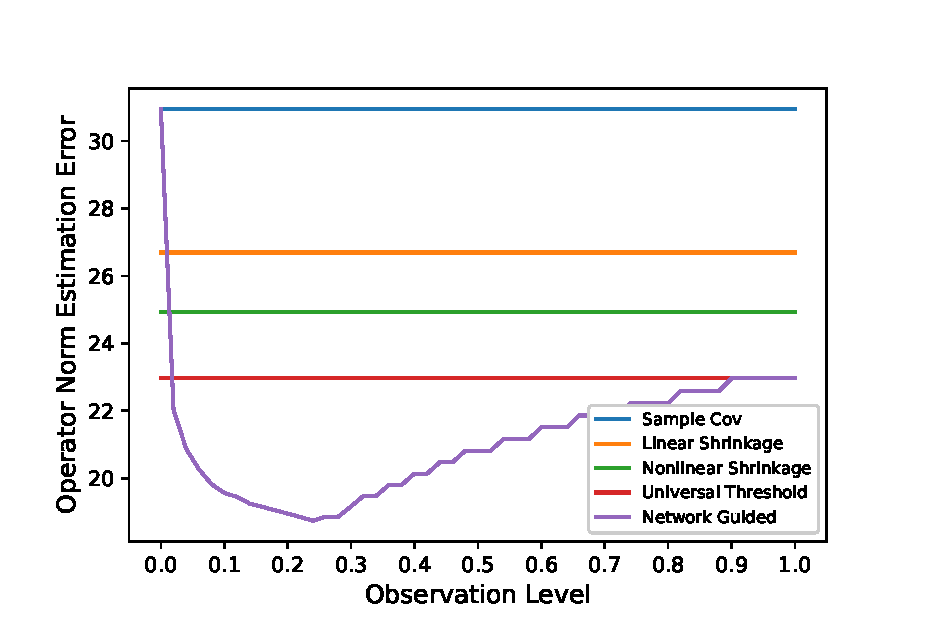
\includegraphics{asset/observation-level-2.eps}
    \caption{The estimation error against the observation level}
    \label{fig:1}
\end{figure}
\begin{figure}
    \centering
    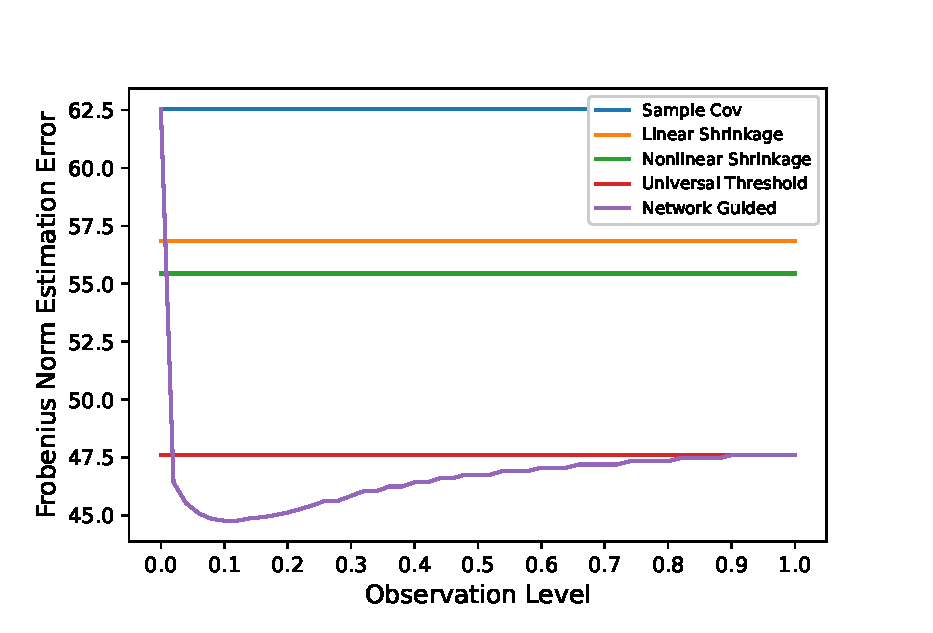
\includegraphics{asset/observation-level-fro.eps}
    \caption{The estimation error against the observation level}
    \label{fig:2}
\end{figure}
\begin{figure}
    \centering
    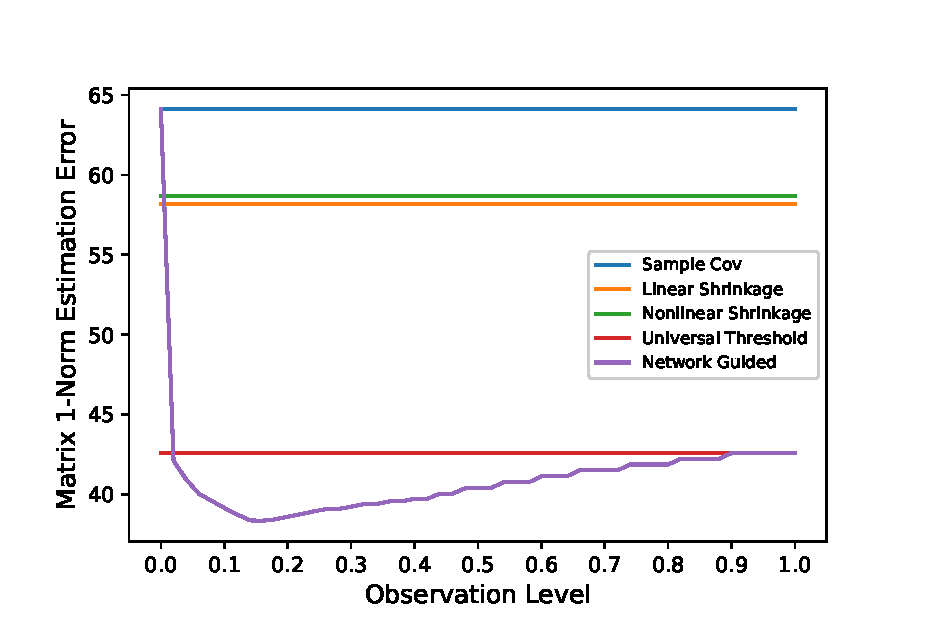
\includegraphics{asset/observation-level-1.eps}
    \caption{The estimation error against the observation level}
    \label{fig:3}
\end{figure}

\begin{longtable}{lrrrrrrrrrrr}
\caption{The estimation error in terms of Operator Norm of the Network Guided Estimator with varying probabilities $p$, $q$ that determine how $G$ is generated.}
\label{t:3-2}\\
\toprule
q &   0.0 &   0.1 &   0.2 &   0.3 &   0.4 &   0.5 &   0.6 &   0.7 &   0.8 &   0.9 &   1.0 \\
p   &       &       &       &       &       &       &       &       &       &       &       \\
\midrule
\endfirsthead
\caption[]{The estimation error in terms of Operator Norm of the Network Guided Estimator with varying probabilities $p$, $q$ that determine how $G$ is generated.} \\
\toprule
q &   0.0 &   0.1 &   0.2 &   0.3 &   0.4 &   0.5 &   0.6 &   0.7 &   0.8 &   0.9 &   1.0 \\
p   &       &       &       &       &       &       &       &       &       &       &       \\
\midrule
\endhead
\midrule
\multicolumn{12}{r}{{Continued on next page}} \\
\midrule
\endfoot

\bottomrule
\endlastfoot
0.0 & 19.74 & 19.94 & 20.11 & 20.49 & 20.92 & 21.42 & 21.81 & 22.41 & 22.99 & 23.62 & 24.32 \\
0.1 & 19.35 & 19.63 & 19.79 & 20.17 & 20.53 & 21.03 & 21.41 & 22.09 & 22.56 & 23.30 & 24.49 \\
0.2 & 18.98 & 19.20 & 19.42 & 19.78 & 20.23 & 20.56 & 21.11 & 21.72 & 22.24 & 23.46 & 24.80 \\
0.3 & 18.68 & 18.84 & 19.16 & 19.49 & 19.81 & 20.33 & 20.70 & 21.43 & 22.39 & 23.80 & 25.21 \\
0.4 & 18.18 & 18.29 & 18.80 & 19.03 & 19.40 & 19.92 & 20.30 & 21.23 & 22.71 & 24.17 & 25.48 \\
0.5 & 17.87 & 18.09 & 18.42 & 18.73 & 19.05 & 19.53 & 20.38 & 21.69 & 23.04 & 24.57 & 25.93 \\
0.6 & 17.48 & 17.81 & 18.02 & 18.45 & 18.94 & 19.52 & 20.63 & 22.01 & 23.53 & 24.91 & 26.25 \\
0.7 & 17.15 & 17.36 & 17.63 & 18.09 & 18.41 & 19.61 & 21.00 & 22.52 & 23.76 & 25.19 & 26.53 \\
0.8 & 16.80 & 16.93 & 17.18 & 17.64 & 18.76 & 20.13 & 21.36 & 22.87 & 24.09 & 25.54 & 26.96 \\
0.9 & 16.42 & 16.65 & 16.99 & 17.84 & 19.20 & 20.48 & 21.84 & 23.22 & 24.43 & 25.92 & 27.26 \\
1.0 & 16.07 & 16.38 & 16.86 & 18.22 & 19.41 & 20.86 & 22.11 & 23.47 & 24.84 & 26.28 & 27.64 \\
\end{longtable}

\begin{longtable}{lrrrrrrrrrrr}
\caption{The estimation error in terms of Frobenius Norm of the Network Guided Estimator with varying probabilities $p$, $q$ that determine how $G$ is generated.}
\label{t:3-fro}\\
\toprule
q &   0.0 &   0.1 &   0.2 &   0.3 &   0.4 &   0.5 &   0.6 &   0.7 &   0.8 &   0.9 &   1.0 \\
p   &       &       &       &       &       &       &       &       &       &       &       \\
\midrule
\endfirsthead
\caption[]{The estimation error in terms of Frobenius Norm of the Network Guided Estimator with varying probabilities $p$, $q$ that determine how $G$ is generated.} \\
\toprule
q &   0.0 &   0.1 &   0.2 &   0.3 &   0.4 &   0.5 &   0.6 &   0.7 &   0.8 &   0.9 &   1.0 \\
p   &       &       &       &       &       &       &       &       &       &       &       \\
\midrule
\endhead
\midrule
\multicolumn{12}{r}{{Continued on next page}} \\
\midrule
\endfoot

\bottomrule
\endlastfoot
0.0 & 47.86 & 49.31 & 50.77 & 52.31 & 53.56 & 54.93 & 56.27 & 57.55 & 58.66 & 59.94 & 61.17 \\
0.1 & 47.44 & 48.86 & 50.43 & 51.77 & 53.18 & 54.47 & 55.75 & 57.02 & 58.36 & 59.59 & 60.82 \\
0.2 & 47.04 & 48.54 & 50.01 & 51.34 & 52.68 & 54.10 & 55.44 & 56.80 & 57.95 & 59.29 & 60.48 \\
0.3 & 46.56 & 47.93 & 49.46 & 51.09 & 52.33 & 53.73 & 55.24 & 56.36 & 57.72 & 58.88 & 60.12 \\
0.4 & 46.07 & 47.50 & 49.28 & 50.54 & 51.96 & 53.37 & 54.73 & 55.90 & 57.48 & 58.54 & 59.82 \\
0.5 & 45.62 & 47.13 & 48.80 & 50.19 & 51.59 & 52.99 & 54.34 & 55.71 & 56.95 & 58.22 & 59.36 \\
0.6 & 45.11 & 46.75 & 48.36 & 49.80 & 51.13 & 52.49 & 54.07 & 55.22 & 56.56 & 57.87 & 59.10 \\
0.7 & 44.68 & 46.24 & 47.94 & 49.17 & 50.66 & 52.11 & 53.50 & 54.98 & 56.15 & 57.43 & 58.72 \\
0.8 & 44.14 & 45.85 & 47.40 & 48.85 & 50.29 & 51.51 & 53.19 & 54.46 & 55.77 & 57.14 & 58.33 \\
0.9 & 43.71 & 45.40 & 46.94 & 48.54 & 49.98 & 51.35 & 52.66 & 54.09 & 55.52 & 56.67 & 57.97 \\
1.0 & 43.23 & 44.96 & 46.41 & 48.01 & 49.47 & 50.98 & 52.25 & 53.73 & 55.04 & 56.37 & 57.62 \\
\end{longtable}

\begin{longtable}{lrrrrrrrrrrr}
\caption{The estimation error in terms of Matrix 1-Norm of the Network Guided Estimator with varying probabilities $p$, $q$ that determine how $G$ is generated.}
\label{t:3-1}\\
\toprule
q &   0.0 &   0.1 &   0.2 &   0.3 &   0.4 &   0.5 &   0.6 &   0.7 &   0.8 &   0.9 &   1.0 \\
p   &       &       &       &       &       &       &       &       &       &       &       \\
\midrule
\endfirsthead
\caption[]{The estimation error in terms of Matrix 1-Norm of the Network Guided Estimator with varying probabilities $p$, $q$ that determine how $G$ is generated.} \\
\toprule
q &   0.0 &   0.1 &   0.2 &   0.3 &   0.4 &   0.5 &   0.6 &   0.7 &   0.8 &   0.9 &   1.0 \\
p   &       &       &       &       &       &       &       &       &       &       &       \\
\midrule
\endhead
\midrule
\multicolumn{12}{r}{{Continued on next page}} \\
\midrule
\endfoot

\bottomrule
\endlastfoot
0.0 & 46.95 & 49.00 & 49.80 & 52.40 & 53.62 & 54.57 & 57.29 & 57.80 & 60.11 & 63.76 & 65.74 \\
0.1 & 46.95 & 47.53 & 49.97 & 51.99 & 53.87 & 53.88 & 55.89 & 58.53 & 60.09 & 62.86 & 65.74 \\
0.2 & 46.61 & 48.19 & 49.71 & 49.79 & 53.39 & 54.74 & 56.73 & 58.43 & 60.45 & 62.75 & 65.16 \\
0.3 & 45.49 & 47.53 & 49.30 & 50.74 & 52.88 & 54.29 & 56.22 & 59.85 & 61.26 & 61.27 & 64.46 \\
0.4 & 45.31 & 48.02 & 47.97 & 49.82 & 50.84 & 52.93 & 56.19 & 56.59 & 58.12 & 61.22 & 64.03 \\
0.5 & 45.80 & 46.56 & 48.61 & 49.28 & 50.60 & 51.76 & 54.87 & 55.77 & 59.02 & 61.72 & 63.86 \\
0.6 & 44.66 & 47.15 & 47.88 & 49.32 & 52.90 & 52.85 & 54.54 & 55.43 & 60.59 & 61.36 & 63.56 \\
0.7 & 44.49 & 45.75 & 46.69 & 49.94 & 49.30 & 52.34 & 54.33 & 57.37 & 58.59 & 60.21 & 63.63 \\
0.8 & 44.32 & 45.04 & 48.23 & 48.84 & 50.29 & 51.54 & 54.58 & 56.66 & 57.01 & 60.45 & 63.01 \\
0.9 & 43.97 & 45.09 & 45.86 & 48.46 & 50.47 & 51.84 & 54.07 & 55.14 & 57.12 & 59.79 & 62.65 \\
1.0 & 43.32 & 44.17 & 46.89 & 47.86 & 49.40 & 51.31 & 53.18 & 54.54 & 58.56 & 59.94 & 62.07 \\
\end{longtable}


\subsection{Proofs}


\begin{proof}[Proof of Theorem 1]
    We have the following decomposition:
    \begin{equation*}
        \norm{T_{\hat{L},\lambda}\pqty{\hat{\Sigma}} - \Sigma } \leq \norm{T_{\hat{L} ,\lambda}(\Sigma) - \Sigma} +\norm{T_{\hat{L}, \lambda}(\hat{\Sigma}) - T_{\hat{L},\lambda}(\Sigma)} = \mathbf{I} + \mathbf{II}
    \end{equation*}
    The first term can be bounded by 
    \begin{align*}
        \mathbf{I} &\leq \max_{i} \sum_{j} \abs{s_{\hat{L}, \lambda}(\sigma_{ij}) - \sigma_{ij}} \\
        &= \max_{i} \sum_{j} \hat{L}_{ij}^{0} \abs{s_{\lambda}(\sigma_{ij}) - \sigma_{ij}}\\
        &= \max_{i} \sum_{j} \bqty{L_{ij}^{0} \abs{s_{\lambda}(\sigma_{ij}) - \sigma_{ij}} + (\hat{L}_{ij}^{0} - L_{ij}^{0})\abs{s_{\lambda}(\sigma_{ij}) - \sigma_{ij}}} \\
        &\leq (1 + o_{p}(1))\max_{i} \sum_{j} \bqty{L_{ij}^{0} \abs{s_{\lambda}(\sigma_{ij}) - \sigma_{ij}}}\\
        &\leq (1 + o_{p}(1))\max_{i} \sum_{j} \bqty{L_{ij}^{0} \abs{\sigma_{ij} \mathbf{1}\Bqty{\sigma_{ij}\leq \lambda} + (s_{\lambda}(\sigma_{ij}) - \sigma_{ij}) \mathbf{1}\Bqty{\sigma_{ij} > \lambda}}}\\
        &\leq (1 + o_{p}(1)) \max_{i} \sum_{j} \bqty{L_{ij}^{0}\abs{\sigma_{ij}}^{q} \lambda^{1 -q}}\\
        &\leq (1 + o_{p}(1)) c_{0}(p) \lambda^{1-q}
    \end{align*}
    And the second term can be bounded similar to \cite{rothman2009GeneralizedThresholding}, 
    \begin{align*}
        \mathbf{II} &\leq  \max_{i} \sum_{j} \bqty{\hat{L}_{ij}^{1} \abs{\hat{\sigma}_{ij} - \sigma_{ij}} + \hat{L}_{ij}^{0} \abs{s_{\lambda}(\hat{\sigma}_{ij}) - s_{\lambda} (\sigma)_{ij}}}\\
        &\leq (1 + o_{p}(1))c_{1}(p)\max_{ij} \abs{\hat{\sigma}_{ij} - \sigma_{ij}} + (1 + o_{p}(1)) \max_{i} \sum_{j} L_{ij}^{0} \abs{s_{\lambda}(\hat{\sigma}_{ij}) - s_{\lambda} (\sigma)_{ij}} \\
        &= O_{p}\pqty{c_{1}(p) \sqrt{\frac{\log N}{T}} + c_{0}(p) \pqty{\lambda^{1-q} + \lambda^{-q} \sqrt{\frac{\log N}{T}}}} \\
    \end{align*}
    Hence we have 
    \begin{align*}
        \norm{T_{\hat{L},\lambda}\pqty{\hat{\Sigma}} - \Sigma } &= O_{p}\pqty{c_{1}(p) \sqrt{\frac{\log N}{T}} + c_{0}(p) \pqty{\lambda^{1-q} + \lambda^{-q} \sqrt{\frac{\log N}{T}}}} \\
        &= O_{p}\pqty{c_{1}(p) \sqrt{\frac{\log N}{T}} + c_{0}(p)\pqty{\frac{\log N}{T}}^{\frac{1-q}{2}}}
    \end{align*}
\end{proof}

\subsection{Data Description: News Implied Network}

The news data are obtained from RavenPack Equity files Dow Jones Edition for the period January 2004 to December 2015. This comprehensive news dataset combines relevant content from multiple sources, including Dow Jones Newswires, Wall Street Journal, and Barron's MarketWatch, which produce the most actively monitored streams of news articles in the financial system. Each unique news story (identified by a unique story ID) tags the companies mentioned in the news by their unique and permanent entity identifier codes (RP\_ENTITX\_ID),  by which we link to stock identifier TICKER and PERMNO.

As as \cite{ge2021news}, we identify links by news co-mentioning. That is, if a piece of business news reports two companies together, they share a link. We do not consider news that co-mention more than two companies since although news they may carry potential information about links, they provide noisier information. We also remove news with topics including analyst recommendations, rating changes, and index movements as these types of news might stack multiple companies together when they actually do not have real links. \autoref{table:news} provides descriptive statistics for RavenPack Equity files Dow Jones Edition dataset during the sample period. Since our comprehensive news dataset combines several sources, given a similar length of sample period, the number of unique news stories is more than ten times larger than that from \cite{scherbina2015economic} and more than eight hundred times than that from \cite{schwenkler2019network}. For link identification purposes, we only use sample news (1) are not about topics mentioned above (2) tag $S\& P$ $500$ companies and (3) mention exactly two companies, which is a subsample of $1,637,256$ unique news stories.

\begin{table}[ht]
    \centering\renewcommand\cellalign{lc}
    \setcellgapes{3pt}\makegapedcells
    \begin{tabular}{|l|l|} \hline
      \makecell{Number of unique news stories} &$88,316,898$\\ 
      \makecell{Number of stories remaining after removing topics including\\ analyst recommendations, ratings changes, and index movements}&$87,841,641$\\
      \hspace{3mm}Of these: &\\
      \hspace{3mm}Number of stories tag sample companies& $8,341,848 $\\
      \hspace{5mm}Of these: &\\
      \hspace{5mm}Number of stories that mention only one company& $5,507,772 \hspace{1mm}(66.03\%)$\\
      \hspace{5mm}Number of stories that mention exactly two companies& $1,637,256 \hspace{1mm}(19.63\%) $ \\
      \hspace{5mm}Number of stories that mention more than two companies&$1,196,820 \hspace{1mm}(14.34\%)$ \\
    \hline\end{tabular}
    \caption{Descriptive statistics for RavenPack Equity files Dow Jones Edition for the period January 2004 to December 2015.}
    \label{table:news}
\end{table}
    
    % \section{Log}% \input{log.tex}
% The End
    \newpage
\printbibliography
\end{document}